\documentclass[ignorenonframetext,10pt]{beamer}
%\documentclass[paper=a4,12pt,version=last,landscape]{scrartcl}

%\usepackage[latin1]{inputenc}
\usepackage[english]{babel}
\usepackage{amsmath,amssymb}
\usepackage{multimedia}
\usepackage{alltt}
\usepackage{multirow}
\usepackage{textcomp}
\usepackage[footnotesize]{subfigure}
\usepackage{graphicx}


\usepackage{pgfplots}
\pgfplotsset{width=7cm,compat=1.3}% <-- moves axis labels near ticklabels (respects tick label widths)
\usepackage{pgfplotstable}



%\usetheme{Berlin}
\usetheme{Darmstadt}
\useoutertheme[subsection=false]{miniframes}
\useoutertheme{smoothbars}
\usefonttheme{structurebold}
%\setbeamertemplate{navigation symbols}{}
\setbeamercovered{invisible}


\title{Helices of RNAs}
\author{\large Jiabin~Huang}
\date{\today}

\institute[ExpBI]{\normalsize
  AG Experimentelle Bioinformatik (Cyanolab)\\
  Institut f\"ur Biologie III\\
  Universit\"at Freiburg}
\subject{Talk based on Giegerich, Voss, Rehmsmeier (2004) ''Abstract
Shapes of RNA'' Nucleic Acids Research Vol. 32 No. 16}
  
  


\begin{document}

\frame{\maketitle}

% frame 2
\begin{frame}
\frametitle{Outline}
   \begin{itemize}
   \item Introducing abstract shapes  %Introduction
   \item Development of a new structure abstraction
   \item Implementation of an algorithm based on the new abstraction
   \item Possible problems                
   \end{itemize}
\end{frame}

% frame 3
\section{Introduction}
\subsection{}
\begin{frame}
\frametitle{Structural components of RNA}
  %\begin{block}
    RNA has different structural components:
    \begin{itemize}
    \item single-stranded regions (SS)
    \item hairpin loops (HL)
    \item stacking regions (SR)
    \item bulges on 5\'{}side (BL) or 3\'{}side (BR)
    \item internal loops (IL)
    \item multiloops (ML). 
    \end{itemize}
  %\end{block}
\end{frame}
  
\begin{frame}
\frametitle{Structural components of RNA}  
\begin{figure}
  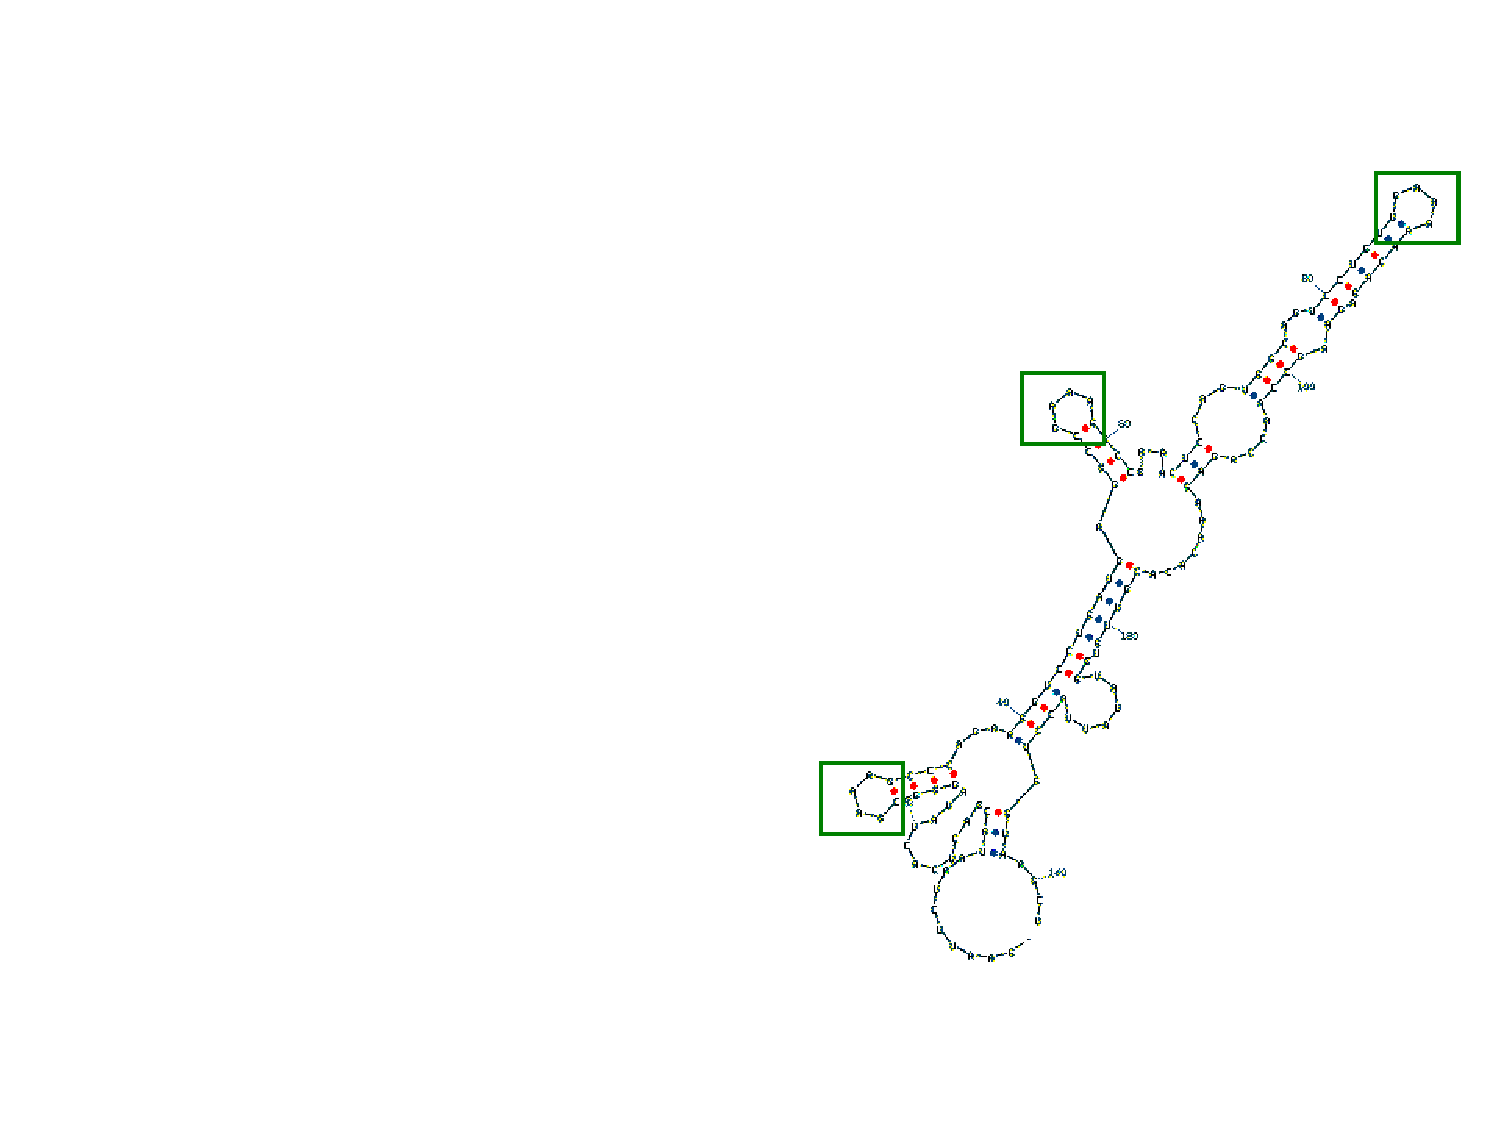
\includegraphics[scale=0.4]{images/structural_components.pdf} 
  \caption{Structural components}
\end{figure}
\end{frame}


% frame 4
% explain the RNA
\begin{frame}
\frametitle{Visualisation of structures}  
\begin{figure}
  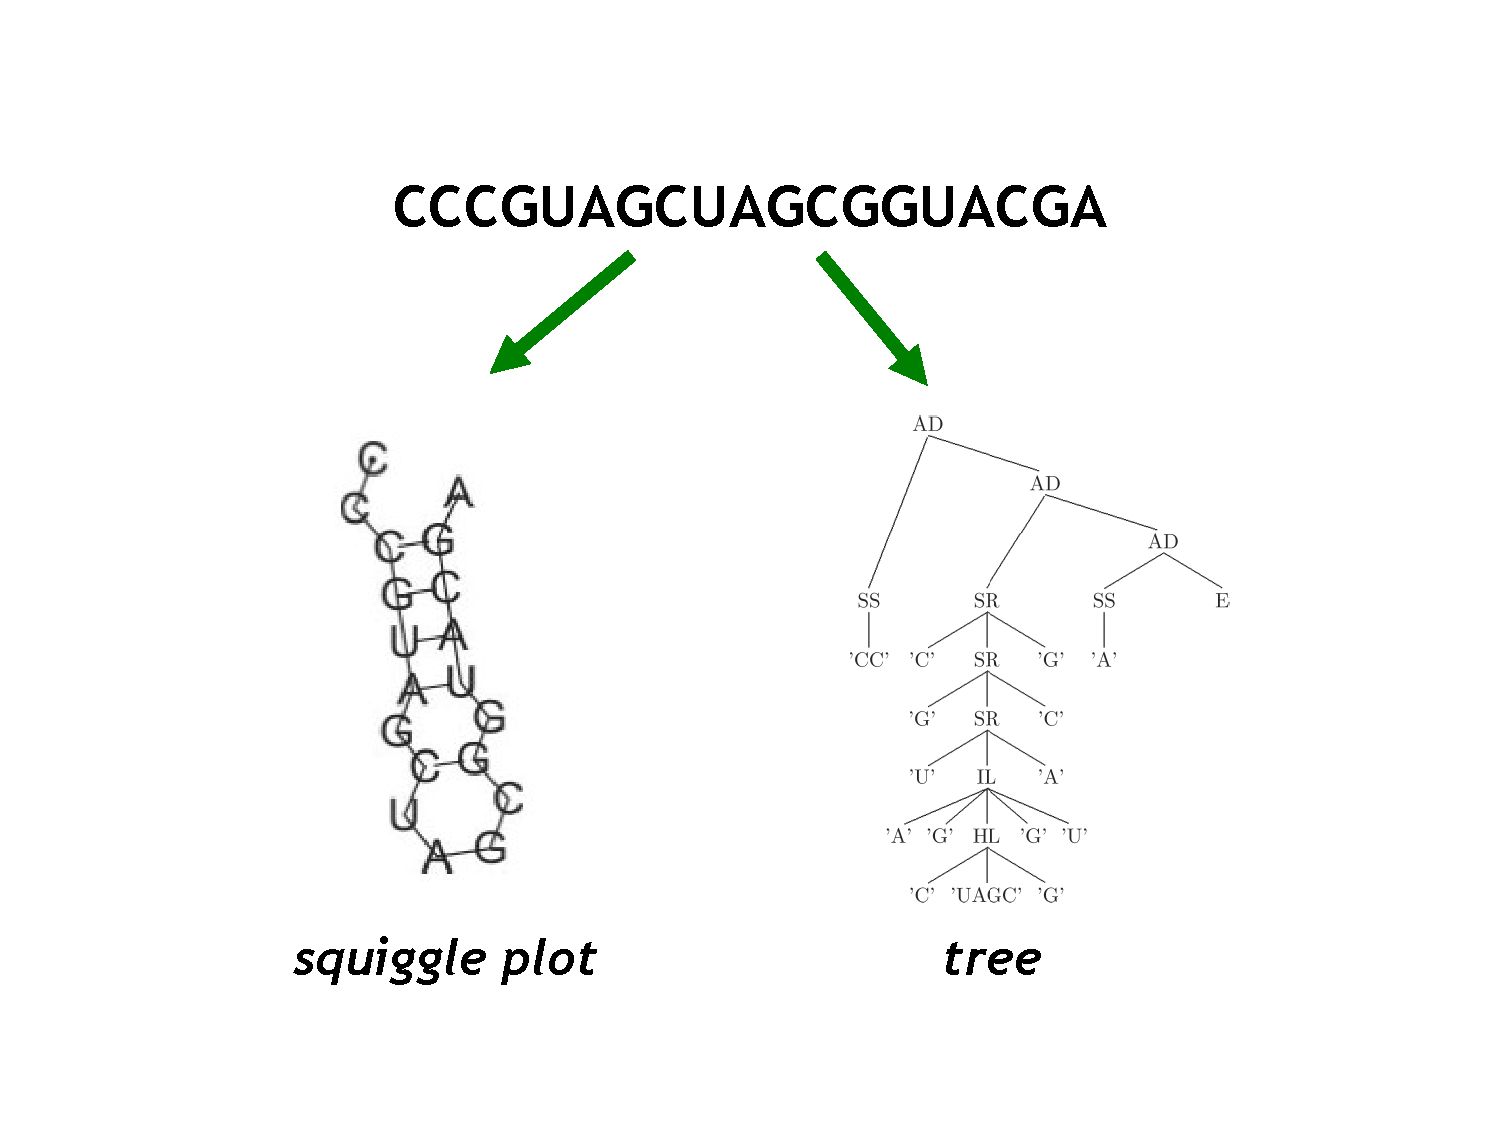
\includegraphics[scale=0.4]{images/visualisation_structures.pdf} 
  %\caption{Structural components}
\end{figure}
\end{frame}

% frame 5
\begin{frame}
\frametitle{Suboptimal structures}
  %\begin{block}
    But the ''true'' structure is not always the one with the lowest
    predicted free energy.
    So what to do?
    \begin{itemize} 
    \item Enumerate suboptimal structures within a given energy range R.
    \item Hope to find a structure fulfilling your expectation or coming close
    to experimental results.
    \end{itemize}
    But the number of suboptimal structures grows exponentially with the energy
    range considered.
  %\end{block}   
\end{frame}

% frame 6
\begin{frame}
\frametitle{Introducing abstract shapes}
    Solution: Use abstract shapes to describe a set of structures.
    \begin{itemize} 
    \item An abstract shape represents a class of similar structures sharing a
    common pattern of helix nesting and adjacency.
    \item ''Abstract'' since we do not care about all details of the structures.
    \item Each shape class has a representative structure called shrep (with minimum folding energy).
    \end{itemize}
\end{frame}

% frame 7
\begin{frame}
\frametitle{Introducing abstract shapes}
    In the domain of shapes, we care only about
    \begin{itemize} 
    \item open structures (OP)
    \item closed structure (CP)
    \item branching (''fork'', FK)
    \item adjacency of structures (AD)
    \end{itemize}
    Level of detail is defined by an abstraction function $\pi$.
    The abstraction function can be defined on the level of the structural components.
\end{frame}

% \begin{frame}
% \frametitle{Defining abstract shapes}
%    \begin{itemize} 
%    \item A (very abstract) abstraction function :
%    \item $\pi$(SS(l))           = OP      (single-stacked region)
%    \item $\pi$(HL(a,l,b)         = CL      (hairpin)
%    \item $\pi$(SR(a,x,b))       = $\pi$(x)                       (stacked region)
%    \item $\pi$(IL(a,l,x,l\'b4,b))  = \'f0(x)       (interior loop)
%    \item $\pi$(ML(a,c,b))       = FK($\pi$(x))                (multiloop) 
%    \item E represents the ``empty structure''.
%    \item where a, b = nucleotides, l = loop, c = list of adjacent 
%    \item components and x = arbitrary structure elements.
%    \end{itemize}
% \end{frame}


% frame 8
\begin{frame}
\frametitle{Example }
\begin{figure}
  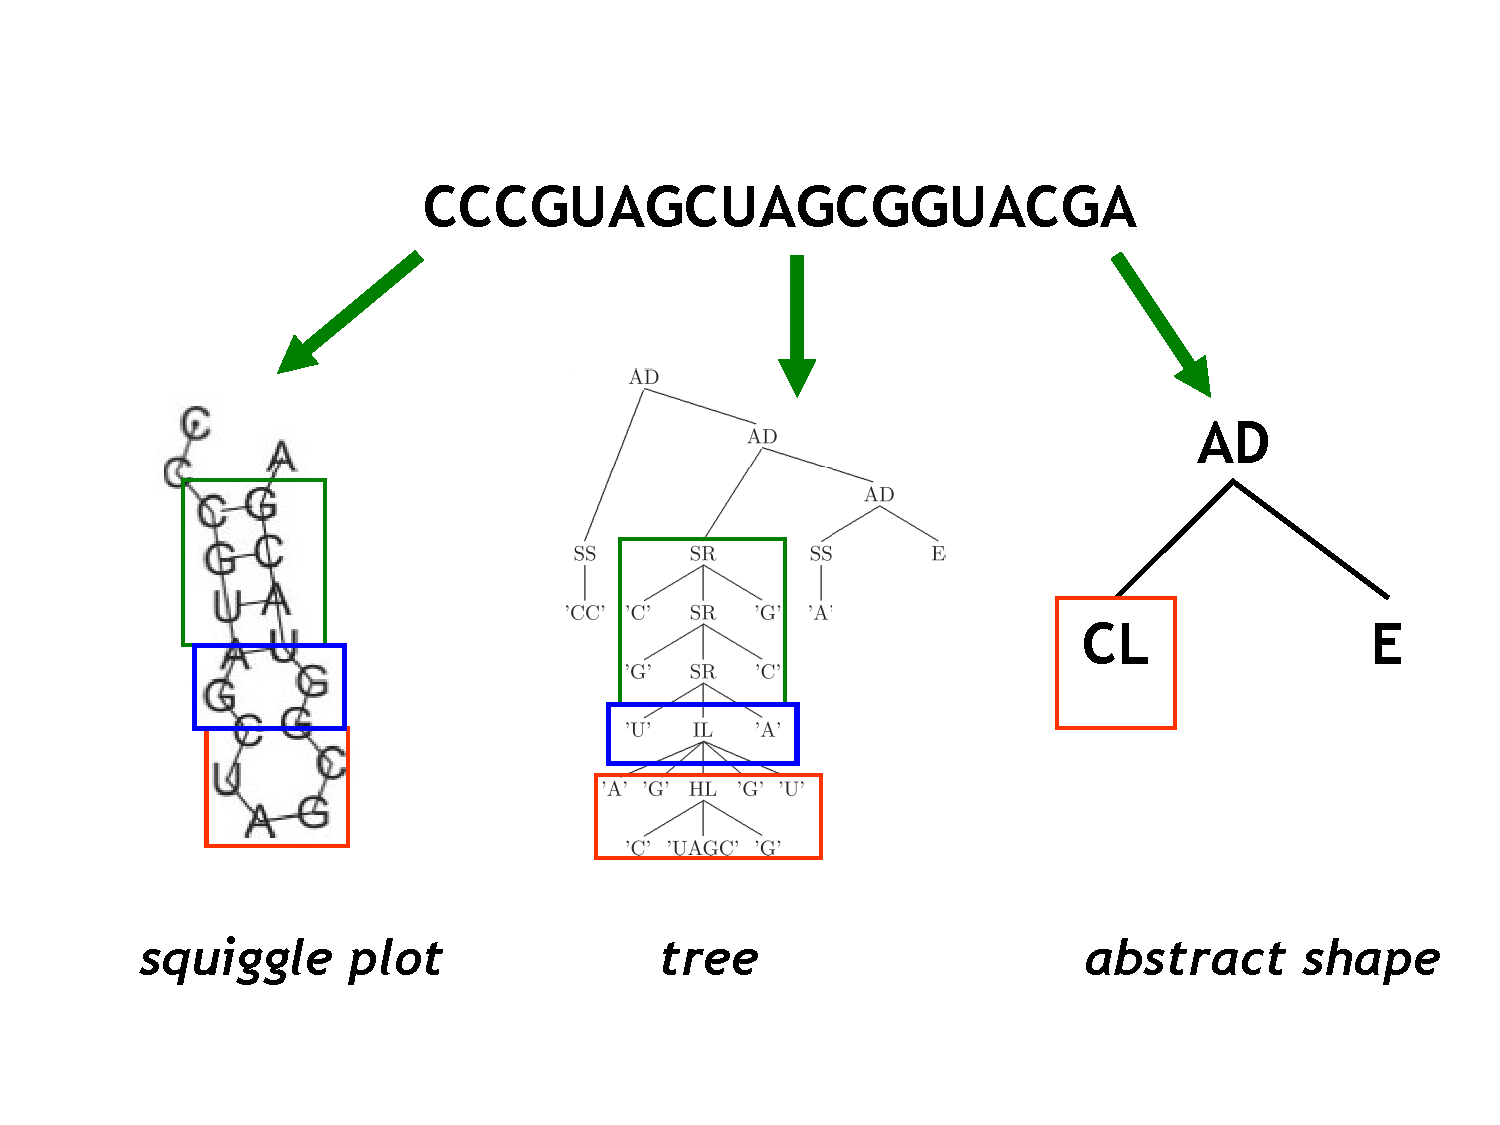
\includegraphics[scale=0.4]{images/shrep_example.pdf} 
\end{figure}
\end{frame}


% frame 9
\begin{frame}[fragile]
  \begin{block}{\small Abstract shape, Energy range: 5 kcal/mol}
  \begin{verbatim}
        UCGCGCACAGGACAUCCUAGGUACAAGGCCGCCGU
-6.30   .((.((..(((....))).(((.....))))))).  [[][]]
-4.90   ........(((....))).(((.....))).....  [][]
-3.90   ....((..(((....)))..)).............  []
  \end{verbatim}
  \end{block}
\end{frame}

% frame 10
\section{develop a new structure abstraction}
\subsection{}
\begin{frame}
\frametitle{}
   \begin{block}{\small Drawback of abstract shape}
   \begin{itemize} 
   \item The major drawback of abstract shape analysis is the position
   independence of the abstraction
   \end{itemize}
   \end{block}
   \begin{block}{\small new algorithm should be:}
   \begin{itemize}
     \item develop a new algorithm for RNA secondary structures which keeps
     track of the position of structural elements
     \item be implemented in the framework of ''Abstract shapes of RNA''
     \item be evaluated and compared to existing algorithms
     \item The new algorithm will be used to design prediction strategies for
     various classes of RNAs
   \end{itemize} 
   \end{block}
\end{frame}


\begin{frame}
\frametitle{develop a new structure abstraction}
    The straightforward idea to overcome the position independence of the
    current available shape abstractions is
    \begin{block}{what keeps track of positions}
    \begin{itemize} 
    \item hairpin loop, because it is the least expensive one
    \item multiloops, as possible braching points, are structurally important    
    \item stacked pairs, bulge and internal loops are the main structural
    contributors 
    \item possible different helices type
    \end{itemize}
    \end{block}
    \begin{block}{which positions of the base pair will be tracked}
    \begin{itemize} 
    \item i
    \item j   
    \item (i,j)
    \item i+j/2
    \end{itemize}    
    \end{block}
\end{frame}


\begin{frame}
\frametitle{Todo: capture of the pdf picture}
\begin{figure}
  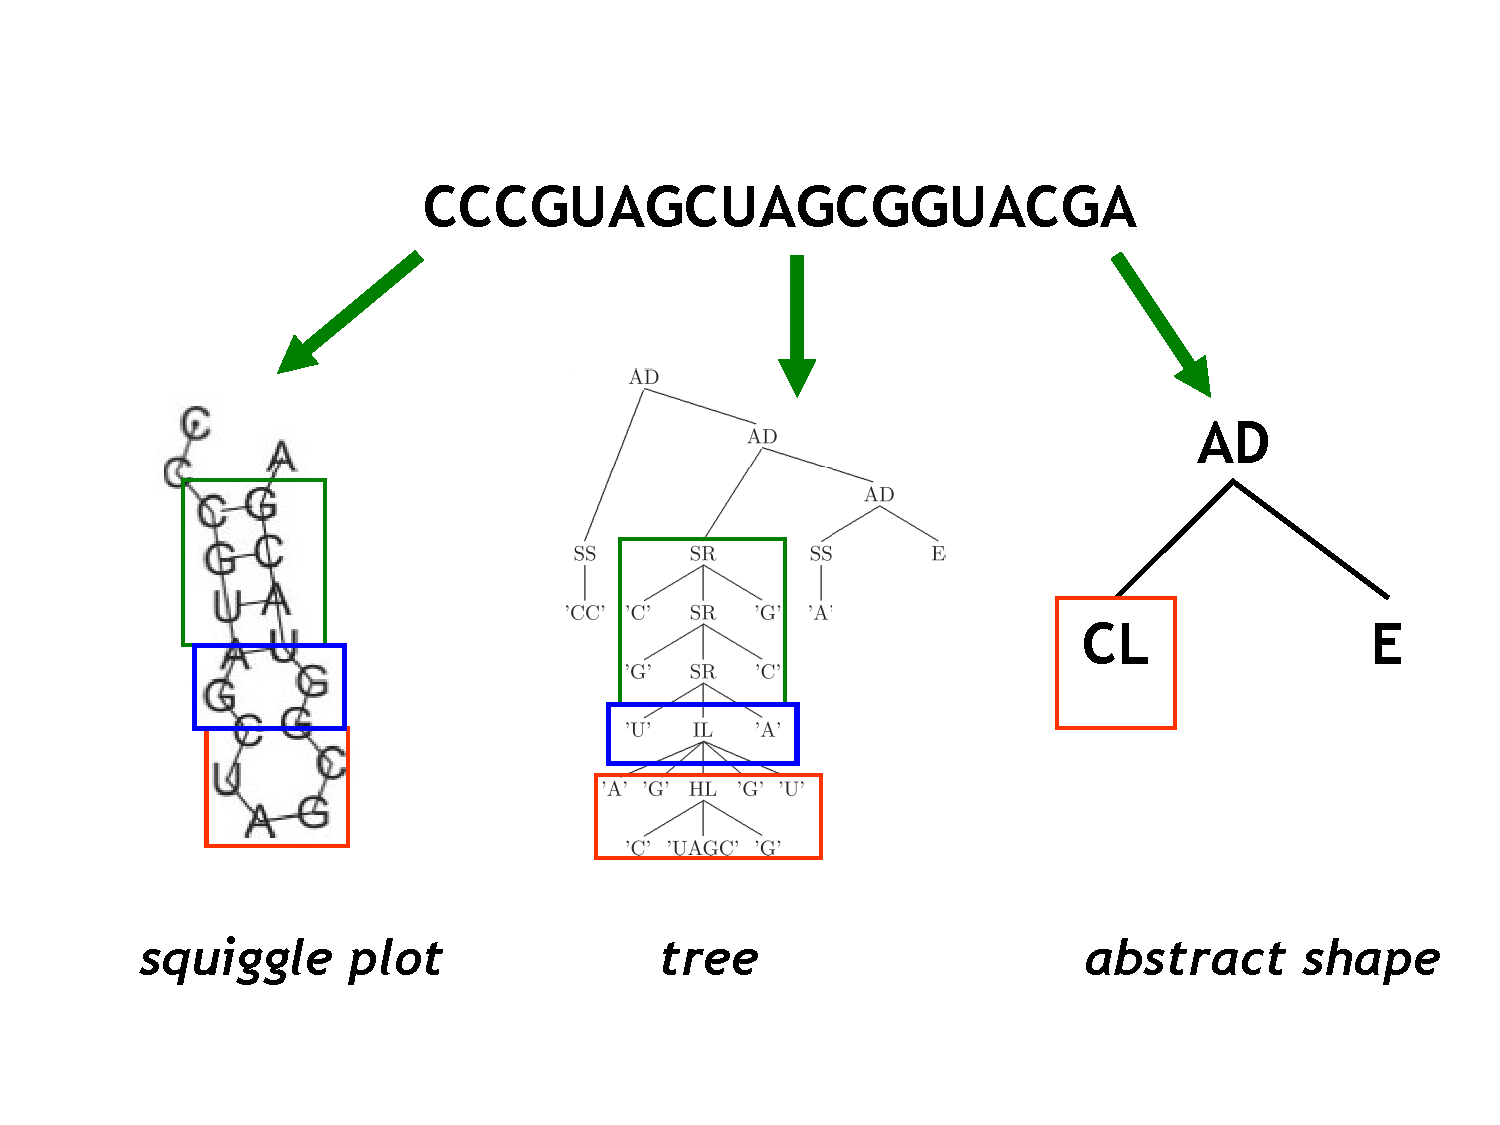
\includegraphics[scale=0.4]{images/shrep_example.pdf} 
\end{figure}
\end{frame}


% frame 11
\begin{frame}[fragile]
  Output from the first trial version of helices shape
  \begin{block}{\small Helices shape, Energy range: 5 kcal/mol}
  %\begin{alltt}
  \begin{verbatim}
        UCGCGCACAGGACAUCCUAGGUACAAGGCCGCCGU
-6.30   .((.((..(((....))).(((.....))))))).  [13.5,25]  
-4.60   ........(((....))).(((........)))..  [13.5,26.5] 
-3.90   ....((..(((....)))..)).............  [13.5]
-3.60   .........((....(((.......)))...))..  [22]
-3.40   ....((..(((....)))..))....((...))..  [13.5,30]
-3.20   ..((((.....((.......)).....)).))...  [17]
-2.80   .........((........(((.....))).))..  [25]
-2.40   ...................(((........)))..  [26.5]
-1.60   ....((..(((....)))..)).....((....))  [13.5,31.5]
  \end{verbatim} 
  %\end{alltt}
  \end{block}
\end{frame}


\begin{frame}
\frametitle{Possible problems}
    \begin{itemize} 
    \item do not preserve nesting of elements and meight lead to abstract shapes
    where a helix index occurs more than once $\rightarrow$ solved with
    different representation form
    \item abstracting from bulge and internal loops might be to rigorous
    $\rightarrow$ refine the definition of the abstraction, such that all critical criteria
    are met
    \item records of helices is a lot more than the records of shapes
    $\rightarrow$ runtime problem  %translation of ..的多
    \end{itemize}
\end{frame}

\begin{frame}
\frametitle{Growth of structure, helix and shape space}
    \centering
	\begin{tikzpicture}
		%\begin{semilogyaxis}[xlabel=Index,ylabel=Value]
		%\addplot gnuplot[color=blue,mark=*]{1.2196*(x**(-1.5))*(2.6180**x)}; 
		%\end{semilogyaxis}
		\begin{semilogyaxis}[legend style={font=\small},xlabel={Sequence
         length},ylabel={Nr. of
         Structures/Helices/Shapes},width=\textwidth,legend style={nodes=right},
         legend pos= north west]
     
        
         \addplot+[only marks,mark=+]
         table[x=X,y=Y]{/home/jhuang/workspace/RNAHeliCes/scripts/estimate_exponent_RNAsubopt.txt};
         \addlegendentry{Structures}         
         \addplot table[x=X,y={create col/linear
         regression={y=Y}}]{/home/jhuang/workspace/RNAHeliCes/scripts/estimate_exponent_RNAsubopt.txt};
         \addlegendentry{$0.33 \cdot x -3.24$}
         
         
         \addplot+[only marks,mark=-]
         table[x=X,y=Y]{/home/jhuang/workspace/RNAHeliCes/scripts/estimate_exponent_RNAhelix.txt};
         \addlegendentry{Helices}         
         \addplot table[x=X,y={create col/linear
         regression={y=Y}}]{/home/jhuang/workspace/RNAHeliCes/scripts/estimate_exponent_RNAhelix.txt};
         \addlegendentry{$0.12 \cdot x +0.36$}
         
  
         \addplot+[only marks,mark=x]
         table[x=X,y=Y]{/home/jhuang/workspace/RNAHeliCes/scripts/estimate_exponent_RNAshapes_5.txt};
         \addlegendentry{Shapes}                   
         \addplot table[x=X,y={create col/linear
         regression={y=Y}}]{/home/jhuang/workspace/RNAHeliCes/scripts/estimate_exponent_RNAshapes_5.txt};                 
         \addlegendentry{
$\pgfmathprintnumber{\pgfplotstableregressiona} \cdot x
\pgfmathprintnumber[print sign]{\pgfplotstableregressionb}$}
         
               
        
        %\addlegendentry{Legenden Eintrag};
        \end{semilogyaxis} 

	\end{tikzpicture}
\end{frame}

\begin{frame}
\frametitle{Outlook: Designing RNA class predictors}
    \begin{itemize} 
    \item specific classes of RNAs, such as riboswitches or miRNA precursors,
    show characteristic features within their folding space
    \item the energy landscape of riboswitches harbors two equally low, but well
    separated minima, but well separated minima
    \item miRNA precursors is governed by one deep and well-defined minimum
    \item develop specialized prediction algorithms for classes of RNAs
    \end{itemize}
\end{frame}

\begin{frame}
\frametitle{End}
   \begin{itemize} 
   \item Thanks a lot for your attention !
   \item Questions ?
   \end{itemize}
\end{frame}


\end{document}
